% An open ball, its boundary, and a sequence in the ball with no limit in the ball.
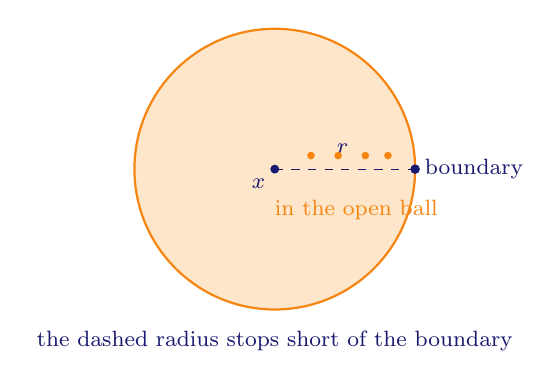
\begin{tikzpicture}[scale=1.15]
  \fill[BurntOrange!18] (0,0) circle (1.55);
  \draw[BurntOrange,thick] (0,0) circle (1.55);
  \fill[MidnightBlue] (0,0) circle (1.4pt) node[below left,font=\footnotesize] {$x$};
  \draw[MidnightBlue,dashed] (0,0)--(1.55,0);
  \node[font=\footnotesize,MidnightBlue] at (0.75,0.22) {$r$};
  \fill[MidnightBlue] (1.55,0) circle (1.5pt) node[right,font=\footnotesize] {boundary};
  \foreach \t/\lab in {0.4/1, 0.7/2, 1.0/3, 1.25/4}{
    \fill[BurntOrange] (\t,0.15) circle (1.2pt);
  }
  \node[font=\footnotesize,BurntOrange] at (0.9,-0.45) {in the open ball};
  \node[font=\footnotesize,MidnightBlue] at (0,-1.9) {the dashed radius stops short of the boundary};
\end{tikzpicture}
